\documentclass{article}
\usepackage{fullpage}
\usepackage{color}
\usepackage[normalem]{ulem}
\usepackage{hyperref}
\usepackage{enumitem}
\usepackage{graphicx}
\hypersetup{colorlinks}
\hyphenpenalty=100000
\begin{document}

\setlength{\voffset}{3.5in}
\title{M3}
\author{\Large Team Sriroku\\
Tom Atnip, George Mammarella, Jeremy Tramm}
\date{\today}
\maketitle
\clearpage
\setlength{\voffset}{0pt}
\tableofcontents
\clearpage


\begin{Large}
\textbf{Changes}
\end{Large}
\\

\begin{tabular}{ | p{1.5in} | p{4.5in} | }
\hline
\textbf{Date} & \textbf{Description}\\
\hline
\hline
March 28, 2013 & Document started\\
\hline
\hline
March 29, 2013 & Title and new lines fixed\\
\hline
\end{tabular}
\clearpage

\section{Development Timeline}
\subsection{End of Week 5}
Generate a valid full board - Tom\\
Pull components and rules together to make a game and display it - Jeremy\\
Difficulty Algorithm - George\\

\subsection{End of Week 6}
Game interface

\subsection{End of  Week 7}
Localization\\
Save/Load Game State\\
User ask for help\\

\subsection{End of Week 8}
Milestone 4 – Metrics\\
Informing of invalidation\\
Rule variations\\

\subsection{End of Week 9}
Milestone 5 – Update Problem Statement\\
Rule variations\\
Wrap-up\\

\subsection{End of Week 10}
Project Due


\section{Coding Standards}
We will be using the native Eclipse Java Programming Standards. 


\section{Class Diagram}

\begin{center}
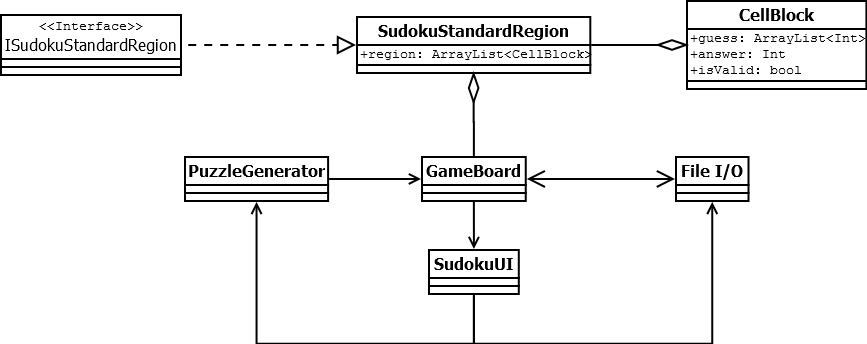
\includegraphics[scale=0.5]{ClassDiagram.png}
\end{center}

\section{Framework and Technology}
Using Java 1.7 and JUnit 4.

\section{References}
Sudoku Puzzles Generating: from Easy to Evil

\end{document}